\documentclass[final]{cpecmu}

%% This is a sample document demonstrating how to use the CPECMU
%% project template. If you are having trouble, see "cpecmu.pdf" for
%% documentation.

\projectNo{P020-2/66}
\acadyear{2023}

\titleTH{ระบบตรวจสอบความหนาแน่นบนรถไฟฟ้าของขนส่งมวลชนมหาวิทยาลัยเชียงใหม่}
\titleEN{Occupancy monitoring system for Chiang Mai University transit electric bus}

\author{นายกิจพิสันต์ ทันงาน}{Chayanon Pitak}{630610716}
\author{นายชญานนท์ พิทักษ์}{Kitpisan Tanngan}{630610724}

\cpeadvisor{paskorn}
\cpecommittee{kampol}
\cpecommittee{santi}

%% Some possible packages to include:
\usepackage[final]{graphicx} % for including graphics

%% Add bookmarks and hyperlinks in the document.
\PassOptionsToPackage{hyphens}{url}
\usepackage[colorlinks=true,allcolors=Blue4,citecolor=red,linktoc=all]{hyperref}
\def\UrlLeft#1\UrlRight{$#1$}

%% Needed just by this example, but maybe not by most reports
\usepackage{afterpage} % for outputting
\usepackage{pdflscape} % for landscape figures and tables. 

%% Some other useful packages. Look these up to find out how to use
%% them.
% \usepackage{natbib}    % for author-year citation styles
% \usepackage{txfonts}
% \usepackage{appendix}  % for appendices on a per-chapter basis
% \usepackage{xtab}      % for tables that go over multiple pages
% \usepackage{subfigure} % for subfigures within a figure
% \usepackage{pstricks,pdftricks} % for access to special PostScript and PDF commands
% \usepackage{nomencl}   % if you have a list of abbreviations

%% if you're having problems with overfull boxes, you may need to increase
%% the tolerance to 9999
% \tolerance=9999

\bibliographystyle{plain}
% \bibliographystyle{IEEEbib}

% \renewcommand{\topfraction}{0.85}
% \renewcommand{\textfraction}{0.1}
% \renewcommand{\floatpagefraction}{0.75}

%% Example for glossary entry
%% Need to use glossary option
%% See glossaries package for complete documentation.
\ifglossary
  \newglossaryentry{lorem ipsum}{
    name=lorem ipsum,
    description={derived from Latin dolorem ipsum, translated as ``pain itself''}
  }
\fi

%% Uncomment this command to preview only specified LaTeX file(s)
%% imported with \include command below.
%% Any other file imported via \include but not specified here will not
%% be previewed.
%% Useful if your report is large, as you might not want to build
%% the entire file when editing a certain part of your report.
% \includeonly{chapters/intro,chapters/background}

\begin{document}
\maketitle
\makesignature

\ifproject
\begin{abstractTH}
    ในระบบขนส่งมวลชนต่างๆ การมีข้อมูลต่างๆ ที่เกี่ยวข้องกับการใช้บริการขนส่งมวลชน จะช่วยให้ผู้ให้บริการขนส่งมวลชนนำข้อมูลที่มีเพื่อจัดการการให้บริการอย่างเหมาะสมและพึงพอใจกับผู้ใช้บริการได้ โดยหนึ่งในข้อมูลที่จำเป็นต่อการให้บริการคือ ความหนาแน่นของผู้โดยสารระหว่างการให้บริการ เราจึงจัดทำ ระบบตรวจสอบความหนาแน่นบนรถไฟฟ้าของขนส่งมวลชนมหาวิทยาลัยเชียงใหม่ ซึ่งเป็นซอฟต์แวร์และชุดอุปกรณ์ที่ตรวจสอบผู้ใช้บริการรถโดยสาร ณ เวลาหนึ่ง, สื่อสารกับระบบที่ผู้พัฒนาโครงการจัดทำขึ้น เพื่อวิเคราห๋และแสดงผลข้อมูลที่ได้จากการวัด
\end{abstractTH}

\begin{abstract}
    In the public transportation system, having various data related to the use of public transportation services will help the service provider manage the service appropriately and satisfy the users. One of the necessary data for service provision is the occupancy during the service. We, therefore, developed a system to check the bus occupancy for the Chiang Mai University transit electric bus. The system is software and a set of devices that check the passenger on the bus at a specific time and communicate with the system developed by the project developer, to analyze and display the data obtained from the measurement.
\end{abstract}

\iffalse
\begin{dedication}
This document is dedicated to all Chiang Mai University students.

Dedication page is optional.
\end{dedication}
\fi % \iffalse

\begin{acknowledgments}
    โครงงานเรื่อง ระบบตรวจสอบความหนาแน่นบนรถไฟฟ้าของขนส่งมวลชนมหาวิทยาลัยเชียงใหม่ เพื่อการสำเร็จการศึกษาของนักศึกษาระดับปริญญาตรี สามารถสำเร็จลุล่วงไปได้ด้วยดี เนื่องจากได้รับความอนุเคราห์จาก ผู้ช่วยศาสตราจารย์ ดร. ภาสกร แช่มประเสริฐ อาจารย์ที่ปรึกษา, ผู้ช่วยศาสตราจารย์ ดร. กําพล วรดิษฐ์, และ รองศาสตราจารย์ ดร. สันติ พิทักษ์กิจนุกูร คณะกรรมการที่ปรึกษาโครงงาน ที่ได้กรุณาให้คำปรึกษา คำแนะนำ ความรู้ และการสนับสนุนอื่นๆ ตลอดระยะเวลาการศึกษา จนโครงงานนี้สามารถสำเร็จลุล่วงไปได้ด้วยดี 

    ขอขอบคุณ ศูนย์บริหารจัดการเมืองอัจฉริยะมหาวิทยาลัยเชียงใหม่ ที่ให้ความอนุเคราะห์ในการให้ข้อมูลการเดินรถของรถไฟฟ้าของขนส่งมวลชนมหาวิทยาลัยเชียงใหม่ รวมถึงอนุเคราห์ให้ติดตั้งชุดอุปกรณ์บนรถไฟฟ้าของขนส่งมวลชนมหาวิทยาลัยเชียงใหม่ชั่วคราว

    ขอขอบคุณกลุ่มงานวิจัย OASYS ที่ให้ความอนุเคราห์อุปกรณ์ต่างๆที่ใช้ในการพัฒนาโครงงาน

    สุดท้ายนี้ผู้พัฒนาโครงงานหวังว่าโครงงานนี้จะเป็นประโยชน์สำหรับสำหรับหน่วยงานที่เกี่ยวข้องและ ผู้ที่สนใจศึกษาต่อไป
\acksign{2024}{3}{25}
\end{acknowledgments}%
\fi % \ifproject

\contentspage

\ifproject
\figurelistpage

\tablelistpage
\fi % \ifproject

% \abbrlist % this page is optional

% \symlist % this page is optional

% \preface % this section is optional


\pagestyle{empty}\cleardoublepage
\normalspacing \setcounter{page}{1} \pagenumbering{arabic} \pagestyle{cpecmu}

\chapter{\ifenglish Introduction\else บทนำ\fi}

\section{\ifenglish Project rationale\else ที่มาของโครงงาน\fi}

ในการให้บริการขนส่งมวลชนในปัจจุบัน ผู้ให้บริการจําเป็นต้องมีข้อมูลเกี่ยวกับบริการที่ถูกต้องและแม่นยํา
ซึ่งหนึ่งในข้อมูลนั้นคือข้อมูลความหนาแน่นของผู้โดยสาร ณ เวลาหนึ่ง ซึ่งบริการรถไฟฟ้าของขนส่งมวลชน
มหาวิทยาลัยเชียงใหม่ก็มีระบบวัดข้อมูลความหนาแน่นเช่นกัน โดยทํางานภายใต้พื้นฐานของการประมวลผล
ภาพจากกล้อง แต่ว่าข้อมูลที่ได้นั้นไม่แม่นยํามากพอ เนื่องจากปัญหาสภาพแวดล้อม ซึ่งไม่สามารถควบคุมได้ ผู้
จัดทําโครงงานจึงต้องการจัดทําระบบใหม่เพื่อเพิ่มความแม่นยําของการเก็บข้อมูลและแสดงผลความหนาแน่นของผู้โดยสารผ่าน
โครงงานนี้

\section{\ifenglish Objectives\else วัตถุประสงค์ของโครงงาน\fi}
\begin{enumerate}
    \item พัฒนาระบบวัดความหนาแน่นของระบบขนส่งมวลชนของรถไฟฟ้าของขนส่งมวลชนมหาวิทยาลัย
    เชียงใหม่ให้แม่นยํามากกว่าระบบที่มีอยู่เดิมและใช้งานได้จริงในสภาพแวดล้อมจริง
    \item พัฒนาระบบวัดความหนาแน่นของรถโดยสารที่มีความแม่นยำสูง และต้นทุนต่ำ
    \item พัฒนาเว็บแอพพลิเคชันที่สามารถแสดงผลข้อมูลความหนาแน่นของผู้โดยสารจากระบบที่พัฒนาข้างต้น
\end{enumerate}

\section{\ifenglish Project scope\else ขอบเขตของโครงงาน\fi}

\subsection{\ifenglish Hardware scope\else ขอบเขตด้านฮาร์ดแวร์\fi}
\begin{enumerate}
    \item อุปกรณ์ที่ใช้สำหรับวัดความหนาแน่นของผู้โดยสารนั้นจะพัฒนาและมดสอบการติดตั้งบนรถไฟฟ้าของขนส่งมวลชนมหาวิทยาลัยเชียงใหม่เท่านั้น ซึ่งเป็นรถไฟฟ้าขนาด 16 ที่นั่ง (ไม่รวมที่นั่งคนขับ) และมีทางเข้าออกของผู้โดยสาร 2 ประตู
    \item อุปกรณ์สําหรับวัดความหนาแน่นจะวัดได้อย่างถูกเฉพาะการโดยสารของมนุษย์ ไม่รวมการโดยสารของ
    สัตว์เลี้ยง หรือวัตถุใดๆที่ไม่ใช่มนุษย์
    \item อุปกรณ์สําหรับวัดความหนาแน่นจะวัดได้อย่างถูกต้องเฉพาะการเข้า-ออกรถโดยสารผ่านประตูสําหรับ
    ผู้โดยสารเท่านั้น โดยต้องเข้า-ออกได้มากที่สุดประตูละ 1 คนต่อครั้ง
    \item ระบบวัดความหนาแน่นที่พัฒนาขั้นจะสามารถทํางานได้ถูกต้องในช่วงเวลาที่รถไฟฟ้าที่ถูกติดตั้งอยู่ในระหว่างการให้บริการ (07:00 น. - 22:00 น.)
    \item พื้นที่อุปกรณ์ที่พัฒนาขึ้นทํางานอยู่จะต้องไม่ถูกรบกวนสัญญาณเซลลูราร์มากเกินกว่า
    ระดับสิ่งแวดล้อมทั่วไป
    \item อุปกรณ์ที่พัฒนาขึ้นจะไม่รบกวนการทำงานใดๆของรถโดยสารที่ถูกติดตั้งอยู่
\end{enumerate}

\subsection{\ifenglish Software scope\else ขอบเขตด้านซอฟต์แวร์\fi}
\begin{enumerate}
    \item เว็บแอพพลิเคชันที่พัฒนาขึ้นจะสามารถแสดงผลข้อมูลความหนาแน่นของผู้โดยสารจากระบบที่พัฒนาข้างต้นเท่านั้น
    \item เว็บแอพพลิเคชันที่พัฒนาขึ้นจะแสดงผลได้อย่างถูกต้องบนเดสก์ท็อปเท่านั้น ไม่รองรับการแสดงผลบนอุปกรณ์พกพาที่ไม่ใช้แลปท็อป
    \item เว็บแอพพลิเคชันที่พัฒนาขึ้นจะสามารถแสดงผลได้อย่างถูกต้องบนเบราว์เซอร์ที่รุ่นสูงกว่า หรือเทียบเท่ากับ Google Chrome รุ่น 45, Firefox รุ่น 34, Safari รุ่น 9, และ Microsoft Edge รุ่น 12 หรือเว็บเบาเซอร์อื่นๆที่การรองรับเทียบเท่ากับเบราว์เซอร์ที่กล่าวมา
\end{enumerate}

\section{\ifenglish Expected outcomes\else ประโยชน์ที่ได้รับ\fi}
\textbf{สำหรับผู้ให้บริการรถโดยสาร}
\begin{enumerate}
    \item สามารถทราบความหนาแน่นของผู้โดยสารในแต่ละคัน, สถานี, สาย และช่วงเวลาได้อย่างแม่นยำโดยไม่ระบุตัวตนของผู้โดยสาร เพื่อนำไปปรับปรุงและพัฒนาระบบโดยสารให้ดียิ่งขึ้น
\end{enumerate}
\textbf{สำหรับผู้รอรถโดยสาร}
\begin{enumerate}
    \item สามารถทราบความหนาแน่นของผู้โดยสารในแต่ละคัน, สถานี และสาย ในปัจจุบันได้ เพื่อนำไปวางแผนการเดินทางตามข้อมูลความหนาแน่นที่ได้รับ
\end{enumerate}

\section{\ifenglish Technology and tools\else เทคโนโลยีและเครื่องมือที่ใช้\fi}

\subsection{\ifenglish Hardware technology\else เทคโนโลยีด้านฮาร์ดแวร์\fi}
\begin{enumerate}
    \item บอร์ดสำหรับพัฒนาระบบสมองกลฝังตัว LilyGo T-A7608E-H ซึ่งเป็นการรวมกันของไมโครคอนโทรลเลอร์ ESP32 ซึ่งเป็นไมโครคอนโทรลเลอร์ที่นิยมใช้ในโครงงานต่างๆ และโมเด็ม SIMCOM A7608E-H สำหรับเชื่อมต่ออินเตอร์เน็ตผ่านเครือข่ายเซลลูลาร์
    \item อุปกรณ์วัดระยะห่างโดยใช้อินฟราเรด Sharp GP2Y0A02YK0F
    \item คอมพิวเตอร์ส่วนตัวสำหรับพัฒนาโปรแกรม
\end{enumerate}

\subsection{\ifenglish Software technology\else เทคโนโลยีด้านซอฟต์แวร์\fi}
\begin{enumerate}
    \item PlatformIO สำหรับการพัฒนาโปรแกรมบนระบบสมองกลฝังตัว
    \item MosquittoMQ สำหรับการรับส่งข้อมูลผ่านโปรโตคอล MQTT
    \item Node.js สำหรับการพัฒนาการเชื่อมต่อระหว่างโบรกเกอร์ MQTT, ฐานข้อมูล และเว็บแอพพลิเคชัน
    \item React.js สำหรับการพัฒนาเว็บแอพพลิเคชัน
\end{enumerate}

\section{\ifenglish Project plan\else แผนการดำเนินงาน\fi}

\textbf{ภาคการศึกษาที่ 2/2565}
\begin{plan}{1}{2022}{3}{2022}
    \planitem{1}{2022}{2}{2022}{ศึกษาค้นคว้าเกี๋ยวกับหัวข้อและข้อมูลต่างๆที่เกี่ยวข้อง}
    \planitem{2}{2022}{3}{2022}{ออกแบบอุปกรณ์สำหรับวัดความหนาแน่น}
    \planitem{2}{2022}{3}{2022}{ออกแบบระบบเชื่อมต่อระหว่างระบบ}
\end{plan}

\textbf{ภาคการศึกษาที่ 2/2566}
\begin{plan}{10}{2023}{3}{2024}
    \planitem{10}{2023}{3}{2024}{ออกแบบอุปกรณ์สำหรับวัดความหนาแน่น}
    \planitem{11}{2023}{3}{2024}{จัดทำอุปกรณ์สำหรับทดสอบ}
    \planitem{12}{2023}{3}{2024}{ทดสอบวัดความหนาแน่นและการส่งข้อมูลบนสภาพแวดล้อมจำลอง}
    \planitem{3}{2024}{3}{2024}{ทดสอบและประเมินผลอุปกรณ์วัดความหนาแน่นและการส่งข้อมูลบนสภาพแวดล้อมจำลองจริง}
    \planitem{10}{2023}{12}{2023}{ออกแบบระบบเชื่อมต่อระหว่างระบบ}
    \planitem{10}{2023}{12}{2023}{ออกแบบประสบการณ์ผู้ใช้และส่วนติดต่อผู้ใช้}
    \planitem{12}{2023}{3}{2024}{พัฒนาเว็บแอพพลิเคชัน}
    \planitem{1}{2024}{3}{2024}{พัฒนาระบบต่างๆบนคลาวด์}
    \planitem{3}{2024}{3}{2024}{ประเมินผลเว็บแอพพลิเคชัน}
    \planitem{3}{2024}{3}{2024}{สรุปผลและจัดทำรายงาน}
\end{plan}

\section{\ifenglish Roles and responsibilities\else บทบาทและความรับผิดชอบ\fi}

นายกิจพิสันต์ ทันงาน รหัสนักศึกษา 630610716 รับผิดชอบในการพัฒนาระบบเชื่อมต่อระหว่างระบบ ฐานข้อมูล และเว็บแอพพลิเคชัน
นายชญานนท์ พิทักษ์ รหัสนักศึกษา 630610724 รับผิดชอบในการพัฒนาอุปกรณ์สำหรับวัดความหนาแน่น
\section{\ifenglish%
Impacts of this project on society, health, safety, legal, and cultural issues
\else%
ผลกระทบด้านสังคม สุขภาพ ความปลอดภัย กฎหมาย และวัฒนธรรม
\fi}

หากโครงการนี้ประสบผลสําเร็จและมีการนําไปต่อยอดแล้ว จะมีผลกระทบต่อการให้บริการรถ
โดยสารต่างๆที่ต้องการข้อมูลความหนาแน่นของผู้โดยสาร เพื่อนำไปพัฒนาการให้บริการที่ตรงต่อความต้องการของผู้ใช้บริการระบบโดยสารมากขึ้นได้ รวมไปถึงให้ผู้ใช้บริการสามารถวางแผยการเดินทางได้อย่างมีประสิทธิภาพมากขึ้น


\chapter{\ifenglish Background Knowledge and Theory\else ทฤษฎีที่เกี่ยวข้อง\fi}

\section{รถรับส่งไฟฟ้าของขนส่งมวลชนมหาวิทยาลัยเชียงใหม่}
  รถรับส่งไฟฟ้าขนาด 16 ที่นั่ง (ไม่รวมคนขับ) 2 ประตู (ไม่รวมประตูฝั่งคนขับ) ที่ให้บริการนักศึกษาและบุคลากรของมหาวิทยาลัยเชียงใหม่ในการไปยังสถานที่ต่างๆระหว่างมหาวิทยาลัยเชียงใหม่
  \begin{figure}[h!]
    \begin{center}
      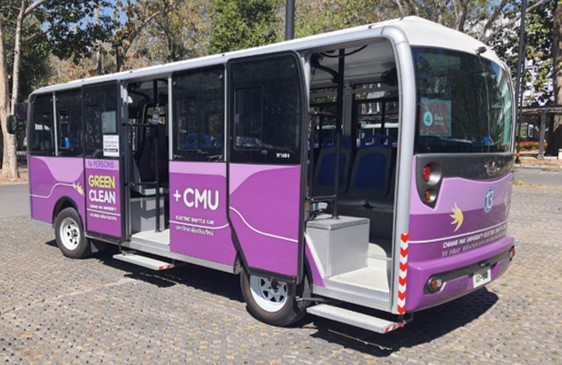
\includegraphics[width=0.5\textwidth]{cmu-evbus.jpg}
    \end{center}
    \caption[Poem]{รถรับส่งไฟฟ้าของขนส่งมวลชนมหาวิทยาลัยเชียงใหม่}
    \label{fig:cmu-ebus}
  \end{figure}

\section{อุปกรณ์วัดระยะห่างโดยใช้อินฟราเรด Sharp GP2Y0A02YK0F}
  \cite[อุปกรณ์วัดระยะห่างโดยใช้อินฟราเรด Sharp GP2Y0A02YK0F]{sharpgp2y0a02yk0f} เป็นอุปกรณ์สำหรับวัดระยะห่างระหว่างตัวอุปกรณ์และวัตถุที่อยู่หน้าอุปกรณ์ ซึ่งการรวมกันของอุปกรณ์ตรวจจับตำแหน่งแสง หรือ Position Sensitive Detector (PSD), ไอโอดแบบเปล่งแสงอินฟราเรด และวงจรประมวลผลสัญญาณหรือ Signal Processing Unit โดยไอโอดแบบเปล่งแสงอินฟราเรด จะเปล่งแสงอินฟราเรดออกไป หากมีวัตถุมาขวางทางของแสง แสงจะสะท้อนกลับมายังอุปกรณ์ตรวจจับตำแหน่งแสงแล้วส่งสัญญาณไปยังวงจรประมวลผลสัญญาณ โดยข้อมูลระยะทางจะส่งในรูปแบบของแรงดันไฟฟ้า ยิ่งวัตถุอยู่ใกล้ จะมีแรงดันไฟฟ้าสูง โดยอุปกรณ์วัดระยะห่างโดยใช้อินฟราเรด Sharp GP2Y0A02YK0F จะสามารถวัดระยะห่างของวัตถุที่มีสีได้ตั้งแต่ 20 เซนติเมตร ไปจนถึง 150 เซนติเมตร
  \begin{figure}[h!]
    \begin{center}
      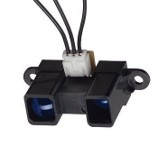
\includegraphics[width=0.25\textwidth]{Sharp-GP2Y0A02YK0F.jpg}
    \end{center}
    \caption[Poem]{อุปกรณ์วัดระยะห่างโดยใช้อินฟราเรด Sharp GP2Y0A02YK0F}
    \label{fig:Sharp-GP2Y0A02YK0F}
  \end{figure}

\section{อุปกรณ์รับ-ส่งข้อมูล GNSS u-blox Neo-7M}
  \cite[อุปกรณ์รับ-ส่งข้อมูล GNSS u-blox Neo-7M]{u-blox-neo-7m} เป็นอุปกรณ์สำหรับรับ-ส่งข้อมูลตำแหน่งทาง GNSS (GPS, GLONASS, QZSS และ SBAS) 
  \begin{figure}[h!]
    \begin{center}
      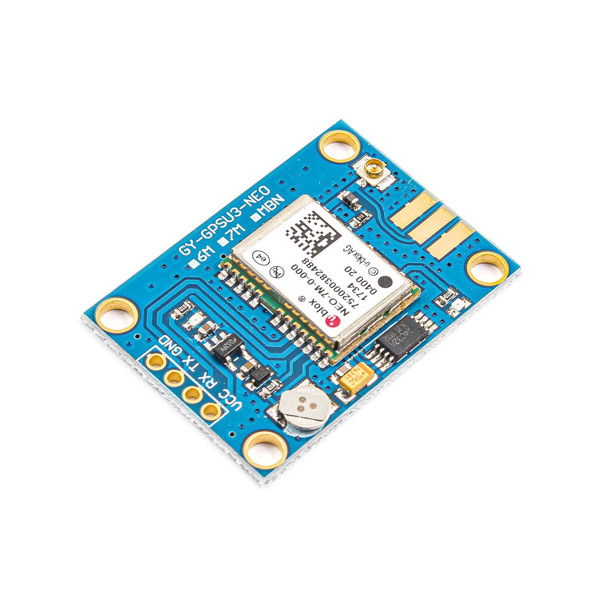
\includegraphics[width=0.25\textwidth]{u-blox-neo-7m.jpg}
    \end{center}
    \caption[Poem]{อุปกรณ์รับ-ส่งข้อมูล GNSS u-blox Neo-7M}
    \label{fig:u-blox-neo-7m}
  \end{figure}

 \section{ไมโครคอรโทรลเลอร์ ESP32}
  \cite[ไมโครคอรโทรลเลอร์ ESP32]{esp32} เป็นไมโครคอนโทรลเลอร์ที่สามารถเชื่อมต่อเครือข่ายไวไฟและบลูทูธได้ และมีความสามารถในการเชื่อมต่อกับอุปกรณ์อื่นๆ ได้หลากหลาย โดยไมโครคอรโทรลเลอร์ ESP32 สามารถเชื่อมต่อกับอุปกรณ์อื่นๆ ผ่านทางอินเทอร์เฟซต่างๆ ได้ เช่น อินเทอร์เฟซ UART, SPI, I2C, GPIO, ADC, DAC, PWM ฯลฯ รวมไปถึงสามารถเขียนโปรแกรมเพื่อควบคุมได้ ทำให้ไมโครคอรโทรลเลอร์ ESP32 มีความสามารถในการทำงานต่างๆ ได้หลากหลาย
  \begin{figure}[h!]
    \begin{center}
      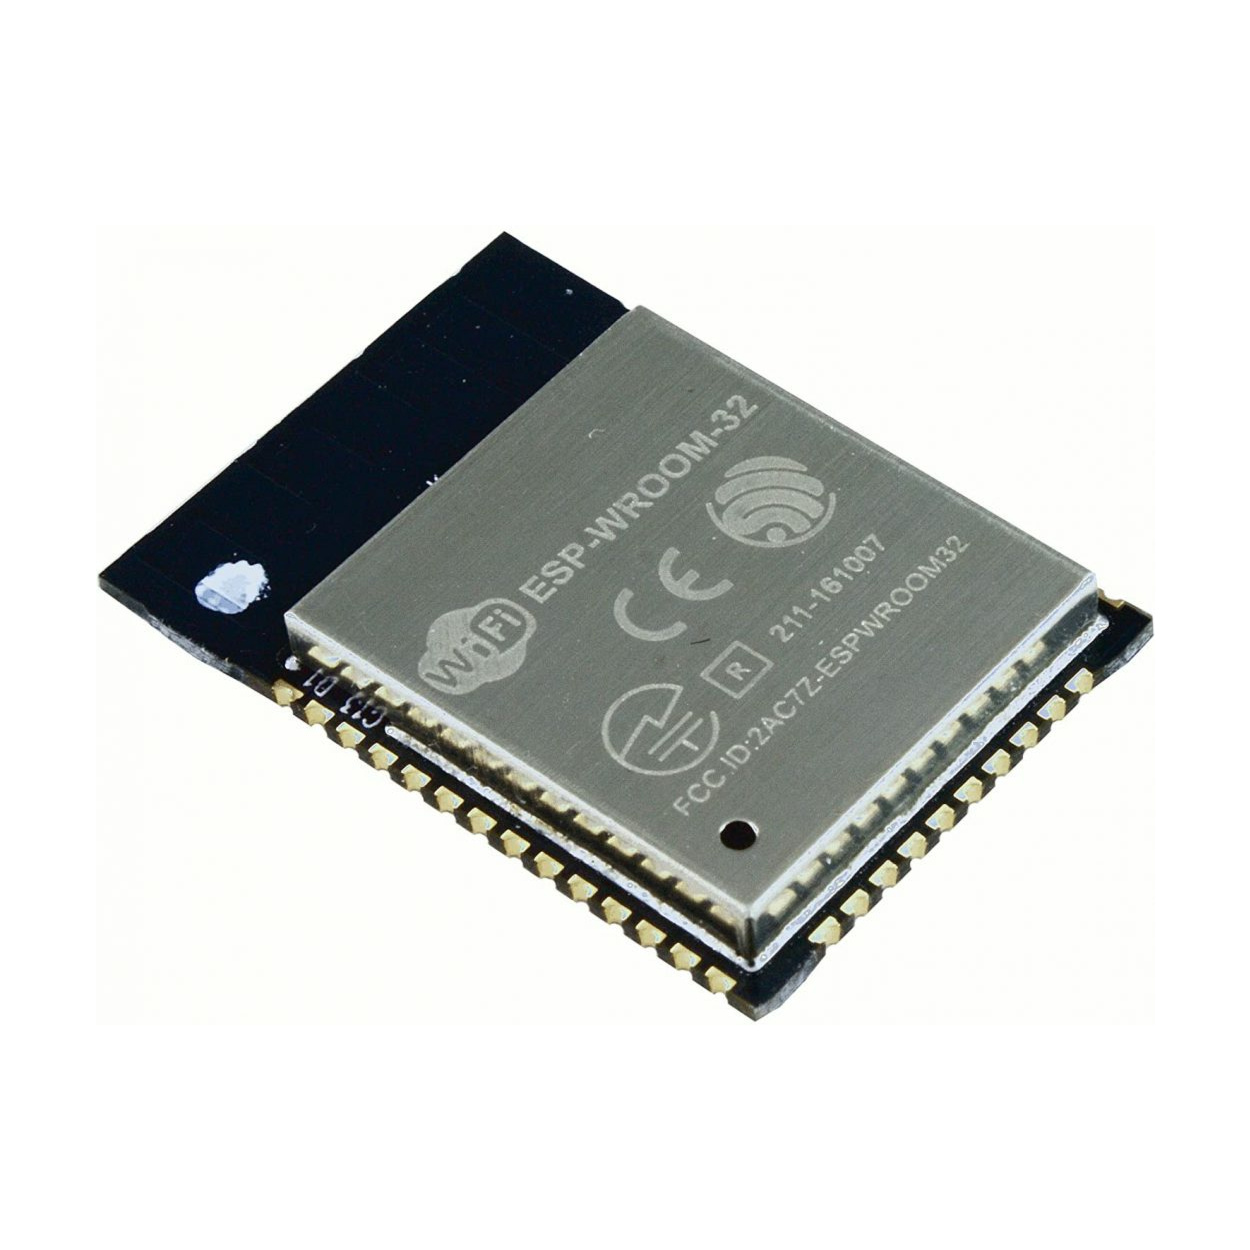
\includegraphics[width=0.25\textwidth]{esp32.png}
    \end{center}
    \caption[Poem]{ไมโครคอรโทรลเลอร์ ESP32}
    \label{fig:esp32}
  \end{figure}

\section{โมเด็ม SIMCOM A7608}
  โมเด็ม SIMCOM A7608 เป็นโมเด็มสำหรับการเชื่อมต่อเครือข่ายไร้สายทั้ง 4G และไวไฟ รวมไปถึงมีอินเตอร์เฟสสำหรับเชื่อมต่อกับโปรโตคอลต่างๆได้ อาทิ MQTT, HTTP ฯลฯ ทำให้สามารถใช้งานโมเด็ม SIMCOM A7608 ในการส่งข้อมูลไปยังเซิร์ฟเวอร์ได้ผ่าน AT Command
  \begin{figure}[h!]
    \begin{center}
      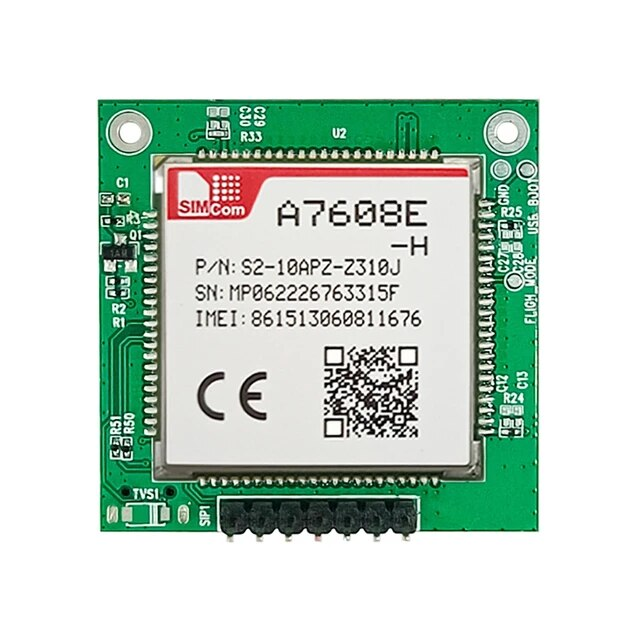
\includegraphics[width=0.25\textwidth]{simcom-a7608e-h.png}
    \end{center}
    \caption[Poem]{โมเด็ม SIMCOM A7608}
    \label{fig:simcom-a7608}
  \end{figure}

\section{บอร์ดสำหรับพัฒนา LILYGO T-A7608}
  บอร์ดสำหรับพัฒนา LILYGO T-A7608 เป็นบอร์ดสำหรับพัฒนาที่รวมเอาความหลากหลายในการทำงานของไมโครคอนโทรลเลอร์ ESP32 และความสามารถในการเชื่อมต่อเครือข่ายไร้สายของ โมเด็ม SIMCOM A-7608 เข้าด้วยกัน ทำให้สามารถใช้งานทั้งสองอุปกรณ์ในการทำงานร่วมกันได้ผ่าน Library ที่ผู้พัฒนาจัดเตรียมไว้ให้
  \begin{figure}[h!]
    \begin{center}
      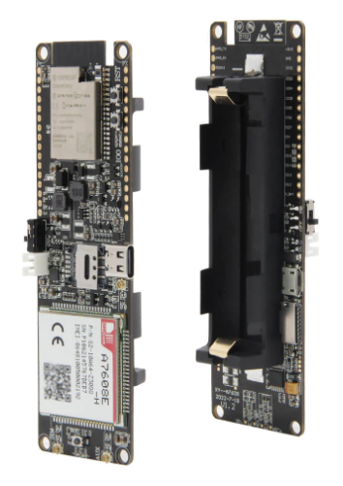
\includegraphics[width=0.25\textwidth]{lilygo-t-a7608.png}
    \end{center}
    \caption[Poem]{บอร์ดสำหรับพัฒนา LILYGO T-A7608}
    \label{fig:lilygo-t-a7608}
  \end{figure}

\section{เครือข่าย LTE}
  \cite[เครือข่าย LTE (Long Term Evolution)]{lte} เป็นเครือข่ายสื่อสารไร้สายที่ใช้ในการสื่อสารข้อมูลระหว่างอุปกรณ์ไร้สาย โดยเครือข่าย LTE สามารถให้ความเร็วในการส่งข้อมูลได้สูงถึง 100 Mbps ในการส่งข้อมูล และ 50 Mbps ในการรับข้อมูล ทำให้เครือข่าย LTE มีความเร็วในการส่งข้อมูลที่สูงกว่าเครือข่ายอื่นๆ ที่ใช้ในการสื่อสารข้อมูลระหว่างอุปกรณ์ไร้สาย รวมไปถึงในปัจจุบัน เครือข่าย LTE ครอบคลุมมากพอที่จะใช้งานในชีวิตแระจำวัน รวมถึงในการพัฒนาโครงงานได้

\section{Global Positioning System}
  Global Positioning System หรือ GPS เป็นระบบดาวเทียมนำร่องโลก เพื่อระบุข้อมูลของตำแหน่งและเวลาโดยอาศัยการคำนวณจากความถี่สัญญาณนาฬิกาที่ส่งมาจากตำแหน่งของดาวเทียมต่างๆ ที่โคจรอยู่รอบโลกทำให้สามารถระบุตำแหน่ง ณ จุดที่สามารถรับสัญญาณได้ทั่วโลกและในทุกสภาพอากาศ รวมถึงสามารถคำนวณความเร็วและทิศทางเพื่อนำมาใช้ร่วมกับแผนที่ในการนำทางได้

\section{โปรโตคอลการส่งข้อมูล HTTP}

\section{โปรโตรคอลการส่งข้อความ MQTT}
  MQTT เป็นโปรโตคอลการส่งข้อความที่อิงตามมาตรฐาน หรือชุดของกฎที่ใช้สําหรับการสื่อสารระหว่าง เครื่องต่อเครื่อง เซ็นเซอร์อัจฉริยะ อุปกรณ์สวมใส่ และอุปกรณ์Internet of Things (IoT) อื่นๆ มักจะ ต้องส่งและรับข้อมูลผ่านเครือข่ายที่มีข้อจํากัดด้านทรัพยากร ซึ่งมีแบนด์วิดท์จํากัด อุปกรณ์IoT เหล่านี้ใช้ MQTT ในการรับส่งข้อมูล เนื่องจากมันใช้งานง่ายและสามารถสื่อสารข้อมูล IoT ได้อย่างมีประสิทธิภาพ MQTT รองรับการส่งข้อความจากอุปกรณ์ไปยังคลาวด์และจากคลาวด์ไปยังอุปกรณ์

\section{โปรโตคอลการส่งข้อความ REST}
  Representational State Transfer (REST) เป็นสถาปัตยกรรมซอฟต์แวร์ที่กําหนดเงื่อนไขว่า API ควร ทํางานอย่างไร โดยแต่แรกเริ่มนั้น มีการสร้าง REST ขึ้นเพื่อเป็นแนวทางในการจัดการการสื่อสารบนเครือ ข่ายที่ซับซ้อน เช่น อินเทอร์เน็ต คุณสามารถใช้สถาปัตยกรรม REST เพื่อรองรับการสื่อสารที่มีประสิทธิภาพ สูงและเชื่อถือได้ในทุกระดับ คุณยังสามารถใช้และปรับเปลี่ยนสถาปัตยกรรมได้อย่างง่ายดาย โดยนําความสามารถในการมองเห็นและการเคลื่อนย้ายข้ามแพลตฟอร์มมาสู่ทุกระบบ API

\section{โบรกเกอร์ MQTT Mosquitto}

\section{Node.js}

\section{influxDB}

\section{React.js}

\section{DigitalOcean Droplet}

\section{\ifenglish%
\ifcpe CPE \else ISNE \fi knowledge used, applied, or integrated in this project
\else%
ความรู้ตามหลักสูตรซึ่งถูกนำมาใช้หรือบูรณาการในโครงงาน
\fi
}
\begin{itemize}
  \item 261102 Computer Programming - พื้นฐานการเขียนโปรแกรมคอมพิวเตอร์
  \item 261207 Basic Computer Engineering Laboratory - พื้นฐานการเขียนเว็บแอพพลิเคชันและการส่งข้อมูล
  \item 252281 Fundamental of Electronics Circuits for ISNE, 261210 Logic and Digital Circuits - การวิเคราห์และออกแบบวงจรดิจิทัล
  \item 261214 Microprocessor and Interfacing - การเขียนโปรแกรมไมโครคอนโทรลเลอร์
  \item 261342 Fundamentals of Database Systems - พื้นฐานการออกแบบและใช้งานฐานข้อมูล
  \item 261441 Internet of Things and Big Data - การส่งข้อมูลและรูปแบบการส่งข้อมูลระหว่างอุปกรณ์อินเตอร์เน็ตในทุกสรรพสิ่งและเครือข่าย
\end{itemize}

\section{\ifenglish%
Extracurricular knowledge used, applied, or integrated in this project
\else%
ความรู้นอกหลักสูตรซึ่งถูกนำมาใช้หรือบูรณาการในโครงงาน
\fi
}
\begin{itemize}
  \item การใช้งานบอร์ดสำหรับพัฒนา LILYGO T-A7608
  \item การใช้งานอุปกรณ์รับ-ส่งข้อมูล GNSS u-blox Neo-7M
  \item การออกแบบระบบบนคลาวด์ที่ใช้ระบบปฏิบัติการ Ubuntu รวมไปถึงการให้บริการระบบต่างๆบนคลาวด์
  \item การออกแบบและจัดการฐานข้อมูลในรูปแบบ Time Series
\end{itemize}
\chapter{\ifproject%
\ifenglish Project Structure and Methodology\else โครงสร้างและขั้นตอนการทำงาน\fi
\else%
\ifenglish Project Structure\else โครงสร้างของโครงงาน\fi
\fi
}

ในบทนี้จะกล่าวถึงหลักการ และการออกแบบระบบ

\makeatletter

% \renewcommand\section{\@startsection {section}{1}{\z@}%
%                                    {13.5ex \@plus -1ex \@minus -.2ex}%
%                                    {2.3ex \@plus.2ex}%
%                                    {\normalfont\large\bfseries}}

\makeatother
%\vspace{2ex}
% \titleformat{\section}{\normalfont\bfseries}{\thesection}{1em}{}
% \titlespacing*{\section}{0pt}{10ex}{0pt}

\section{Alice in Wonderland}

\begin{figure}
\begin{center}
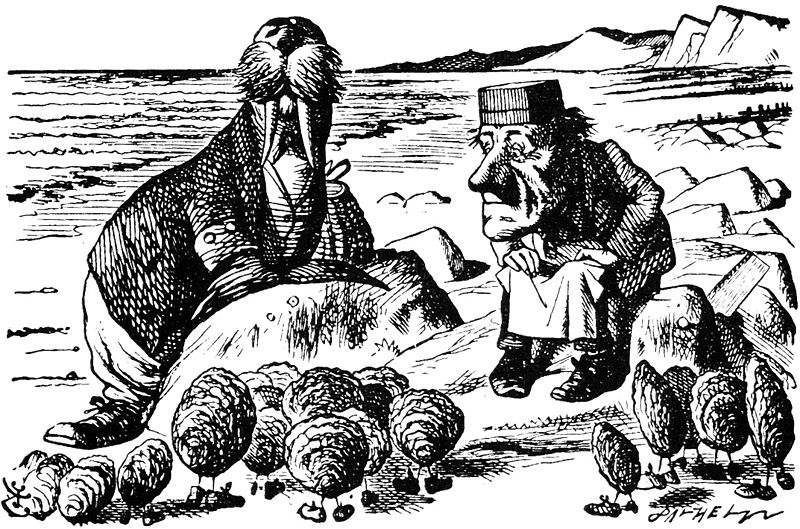
\includegraphics{800px-Briny_Beach.jpg}
\end{center}
\caption[Poem]{The Walrus and the Carpenter}
\label{fig:walrus}
\end{figure}

\subsection{The Black Kitten}
  One thing was certain, that the WHITE kitten had had nothing to
do with it:---it was the black kitten's fault entirely~\cite{aiw}.  For the
white kitten had been having its face washed by the old cat for
the last quarter of an hour (and bearing it pretty well,
considering); so you see that it COULDN'T have had any hand in
the mischief.

  The way Dinah washed her children's faces was this:  first she
held the poor thing down by its ear with one paw, and then with
the other paw she rubbed its face all over, the wrong way,
beginning at the nose:  and just now, as I said, she was hard at
work on the white kitten, which was lying quite still and trying
to purr---no doubt feeling that it was all meant for its good.

  But the black kitten had been finished with earlier in the
afternoon, and so, while Alice was sitting curled up in a corner
of the great arm-chair, half talking to herself and half asleep,
the kitten had been having a grand game of romps with the ball of
worsted Alice had been trying to wind up, and had been rolling it
up and down till it had all come undone again; and there it was,
spread over the hearth-rug, all knots and tangles, with the
kitten running after its own tail in the middle.

\subsection{The Reproach}

  `Oh, you wicked little thing!' cried Alice, catching up the
kitten, and giving it a little kiss to make it understand that it
was in disgrace.  `Really, Dinah ought to have taught you better
manners!  You OUGHT, Dinah, you know you ought!' she added,
looking reproachfully at the old cat, and speaking in as cross a
voice as she could manage---and then she scrambled back into the
arm-chair, taking the kitten and the worsted with her, and began
winding up the ball again.  But she didn't get on very fast, as
she was talking all the time, sometimes to the kitten, and
sometimes to herself.  Kitty sat very demurely on her knee,
pretending to watch the progress of the winding, and now and then
putting out one paw and gently touching the ball, as if it would
be glad to help, if it might.

  `Do you know what to-morrow is, Kitty?' Alice began.  `You'd
have guessed if you'd been up in the window with me---only Dinah
was making you tidy, so you couldn't.  I was watching the boys
getting in stick for the bonfire---and it wants plenty of
sticks, Kitty!  Only it got so cold, and it snowed so, they had
to leave off.  Never mind, Kitty, we'll go and see the bonfire
to-morrow.'  Here Alice wound two or three turns of the worsted
round the kitten's neck, just to see how it would look:  this led
to a scramble, in which the ball rolled down upon the floor, and
yards and yards of it got unwound again.

  `Do you know, I was so angry, Kitty,' Alice went on as soon as
they were comfortably settled again, `when I saw all the mischief
you had been doing, I was very nearly opening the window, and
putting you out into the snow!  And you'd have deserved it, you
little mischievous darling!  What have you got to say for
yourself?  Now don't interrupt me!' she went on, holding up one
finger.  `I'm going to tell you all your faults.  Number one:
you squeaked twice while Dinah was washing your face this
morning.  Now you can't deny it, Kitty:  I heard you!  What that
you say?' (pretending that the kitten was speaking.)  `Her paw
went into your eye?  Well, that's YOUR fault, for keeping your
eyes open---if you'd shut them tight up, it wouldn't have
happened.  Now don't make any more excuses, but listen!  Number
two:  you pulled Snowdrop away by the tail just as I had put down
the saucer of milk before her!  What, you were thirsty, were you?

\chapter{\ifproject%
\ifenglish Experimentation and Results\else การทดลองและผลลัพธ์\fi
\else%
\ifenglish System Evaluation\else การประเมินระบบ\fi
\fi}

ในบทนี้จะกล่าวถึงผลการทดลองจากการวัดผลส่วนต่างๆของโครงงาน ดังนี้

\section{ส่วนอุปกรณ์วัดความหนาแน่น}

โดยได้ติดตั้งอุปกรณ์ทดสอบบนรถไฟฟ้าของขนส่งมวลชนมหาวิทยาลัยเชียงใหม่ ในช่วงวันที่ 25 มีนาคม 2567 ถึงวันที่ 29 มีนาคม 2567 โดยติดตั้งบนรถสายที่ 3 หมายเลข 33 มีเวลาให้บริการตั้งแต่ 09:10 น. ถึง 22:00 น.

\subsection{ความแม่นยำของข้อมูล}

เปรียบเทียบข้อมูลที่ได้จากระบบเทียบกับข้อมูลจริงของผู้โดยสาร โดยการนั่งโดยสารและนับความหนาแน่นจริงบนรถโดยสาร เทียบกับค่าที่ขึ้นในระบบ ทดสอบกับช่วงเวลา 2 ชั่วโมงโดยประมาณ เป็นเวลา 2 วัน โดยมีผลการทดลองดังนี้

\subsubsection{วันที่ 27 มีนาคม 2567}
    \textbf{เวลา 12:35 น.}
    {\tiny\begin{center}
        \begin{tabular}{ | c | c | c | c | c | c | c | c | c | c | c | c | c |  }
            \hline
                \multirow{2}{*}{สถานี} & \multicolumn{3}{|c|}{ความหนาแน่นจริง (คน)} & \multicolumn{3}{|c|}{ความหนาแน่นบนระบบ (คน)} & \multicolumn{3}{|c|}{ผลต่าง (คน)} & \multicolumn{3}{|c|}{ร้อยละที่คลาดเคลื่อน (\%)} \\
            \hline
                & เข้า & ออก & ปัจจุบัน & เข้า & ออก & ปัจจุบัน & เข้า & ออก & ปัจจุบัน & เข้า & ออก & ปัจจุบัน \\
            \hline
                สถานีกลางรถไฟฟ้า ขสมช.            & 4 & 0 & 4 & 3 & 0 & 3 & 1 & 0 & 1 & 6.25 & 0 & 6.25 \\
                อาคารปฏิบัติการกลางคณะวิทยาศาสตร์    & 6 & 0 & 6 & 4 & 0 & 4 & 2 & 0 & 2 & 12.5 & 0 & 12.5 \\
                โรงอาหารคณะรัฐศาสตร์ (ตรงข้าม)*     & 6 & 4 & 2 & 4 & 0 & 4 & 2 & 4 & 2 & 12.5 & 25 & 12.5 \\
                ไปรษณีย์                          & 6 & 4 & 2 & 4 & 0 & 4 & 2 & 4 & 2 & 12.5 & 25 & 12.5 \\ 
                ลานจอดรถ อ่างแก้ว                  & 6 & 4 & 2 & 4 & 0 & 4 & 2 & 4 & 2 & 12.5 & 25 & 12.5 \\
                โรงอาหารคณะมนุษยศาสตร์            & 6 & 4 & 2 & 4 & 0 & 4 & 2 & 4 & 2 & 12.5 & 25 & 12.5 \\
                อาคาร HB7 คณะมนุษยศาสตร์          & 6 & 6 & 0 & 4 & 1 & 3 & 2 & 5 & 3 & 12.5 & 31.25 & 18.75 \\
                สำนักหอสมุด                       & 6 & 6 & 0 & 4 & 1 & 3 & 2 & 5 & 3 & 12.5 & 31.25 & 18.75 \\
                สถานีกลางรถไฟฟ้า ขสมช.            & 6 & 6 & 0 & 4 & 1 & 3 & 2 & 5 & 3 & 12.5 & 31.25 & 18.75 \\
            \hline
        \end{tabular}
    \end{center}}
    * ตั้งค่าสถานีผิด จึงทำให้ค่าความหนาแน่นบนระบบไม่ถูกต้อง ได้แก้ไขแล้วในรอบถัดไป

    \textbf{เวลา 12:55 น.}
    {\tiny\begin{center}
        \begin{tabular}{ | c | c | c | c | c | c | c | c | c | c | c | c | c |  }
            \hline
                \multirow{2}{*}{สถานี} & \multicolumn{3}{|c|}{ความหนาแน่นจริง (คน)} & \multicolumn{3}{|c|}{ความหนาแน่นบนระบบ (คน)} & \multicolumn{3}{|c|}{ผลต่าง (คน)} & \multicolumn{3}{|c|}{ร้อยละที่คลาดเคลื่อน (\%)} \\
            \hline
                & เข้า & ออก & ปัจจุบัน & เข้า & ออก & ปัจจุบัน & เข้า & ออก & ปัจจุบัน & เข้า & ออก & ปัจจุบัน \\
            \hline
                สถานีกลางรถไฟฟ้า ขสมช.            & 0 & 0 & 0 & 0 & 0 & 0 & 0 & 0 & 0 & 0 & 0 & 0 \\
                อาคารปฏิบัติการกลางคณะวิทยาศาสตร์    & 0 & 0 & 0 & 0 & 0 & 0 & 0 & 0 & 0 & 0 & 0 & 0 \\
                โรงอาหารคณะรัฐศาสตร์ (ตรงข้าม)      & 0 & 0 & 0 & 0 & 0 & 0 & 0 & 0 & 0 & 0 & 0 & 0 \\
                ไปรษณีย์                          & 0 & 0 & 0 & 0 & 0 & 0 & 0 & 0 & 0 & 0 & 0 & 0 \\
                ลานจอดรถ อ่างแก้ว                  & 0 & 0 & 0 & 0 & 0 & 0 & 0 & 0 & 0 & 0 & 0 & 0 \\
                โรงอาหารคณะมนุษยศาสตร์            & 0 & 0 & 0 & 0 & 0 & 0 & 0 & 0 & 0 & 0 & 0 & 0 \\
                อาคาร HB7 คณะมนุษยศาสตร์          & 0 & 0 & 0 & 0 & 0 & 0 & 0 & 0 & 0 & 0 & 0 & 0 \\
                สำนักหอสมุด                       & 0 & 0 & 0 & 0 & 0 & 0 & 0 & 0 & 0 & 0 & 0 & 0 \\
                สถานีกลางรถไฟฟ้า ขสมช.            & 0 & 0 & 0 & 0 & 0 & 0 & 0 & 0 & 0 & 0 & 0 & 0 \\
            \hline
        \end{tabular}
    \end{center}}

    \textbf{เวลา 13:15 น.}
    {\tiny\begin{center}
        \begin{tabular}{ | c | c | c | c | c | c | c | c | c | c | c | c | c |  }
            \hline
                \multirow{2}{*}{สถานี} & \multicolumn{3}{|c|}{ความหนาแน่นจริง (คน)} & \multicolumn{3}{|c|}{ความหนาแน่นบนระบบ (คน)} & \multicolumn{3}{|c|}{ผลต่าง (คน)} & \multicolumn{3}{|c|}{ร้อยละที่คลาดเคลื่อน (\%)} \\
            \hline
                & เข้า & ออก & ปัจจุบัน & เข้า & ออก & ปัจจุบัน & เข้า & ออก & ปัจจุบัน & เข้า & ออก & ปัจจุบัน \\
            \hline
                สถานีกลางรถไฟฟ้า ขสมช.            & 1 & 0 & 1 & 0 & 0 & 0 & 1 & 0 & 1 & 6.25 & 0 & 6.25 \\
                อาคารปฏิบัติการกลางคณะวิทยาศาสตร์    & 1 & 0 & 1 & 0 & 0 & 0 & 1 & 0 & 1 & 6.25 & 0 & 6.25 \\
                โรงอาหารคณะรัฐศาสตร์ (ตรงข้าม)      & 1 & 0 & 1 & 0 & 0 & 0 & 1 & 0 & 1 & 6.25 & 0 & 6.25 \\
                ไปรษณีย์                          & 1 & 0 & 1 & 0 & 0 & 0 & 1 & 0 & 1 & 6.25 & 0 & 6.25 \\
                ลานจอดรถ อ่างแก้ว                  & 1 & 0 & 1 & 0 & 0 & 0 & 1 & 0 & 1 & 6.25 & 0 & 6.25 \\
                โรงอาหารคณะมนุษยศาสตร์            & 1 & 0 & 1 & 0 & 0 & 0 & 1 & 0 & 1 & 6.25 & 0 & 6.25 \\
                อาคาร HB7 คณะมนุษยศาสตร์          & 1 & 0 & 1 & 0 & 0 & 0 & 1 & 0 & 1 & 6.25 & 0 & 6.25 \\
                สำนักหอสมุด                       & 1 & 1 & 0 & 0 & 0 & 0 & 0 & 1 & 0 & 0 & 6.25 & 0 \\
                สถานีกลางรถไฟฟ้า ขสมช.            & 1 & 1 & 0 & 0 & 0 & 0 & 0 & 1 & 0 & 0 & 6.25 & 0 \\
            \hline
        \end{tabular}
    \end{center}}

    เฉลี่ยแล้วกิจกรรมการเข้า-ออกรวมคลาดเคลื่อนเฉลี่ยร้อยละ \textbf{1.89} และ จำนวนผู้โดยสารบนรถคลาดเคลื่อนเฉลี่ยร้อยละ \textbf{6.25}

\subsubsection{วันที่ 28 มีนาคม 2567}
    \textbf{เวลา 09:00 น.}
    {\tiny\begin{center}
        \begin{tabular}{ | c | c | c | c | c | c | c | c | c | c | c | c | c |  }
            \hline
                \multirow{2}{*}{สถานี} & \multicolumn{3}{|c|}{ความหนาแน่นจริง (คน)} & \multicolumn{3}{|c|}{ความหนาแน่นบนระบบ (คน)} & \multicolumn{3}{|c|}{ผลต่าง (คน)} & \multicolumn{3}{|c|}{ร้อยละที่คลาดเคลื่อน (\%)} \\
            \hline
                & เข้า & ออก & ปัจจุบัน & เข้า & ออก & ปัจจุบัน & เข้า & ออก & ปัจจุบัน & เข้า & ออก & ปัจจุบัน \\
            \hline
                สถานีกลางรถไฟฟ้า ขสมช.            & 0 & 0 & 0 & 0 & 0 & 0 & 0 & 0 & 0 & 0 & 0 & 0 \\
                อาคารปฏิบัติการกลางคณะวิทยาศาสตร์    & 0 & 0 & 0 & 0 & 0 & 0 & 0 & 0 & 0 & 0 & 0 & 0 \\
                โรงอาหารคณะรัฐศาสตร์ (ตรงข้าม)      & 0 & 0 & 0 & 0 & 0 & 0 & 0 & 0 & 0 & 0 & 0 & 0 \\
                ไปรษณีย์                          & 0 & 0 & 0 & 0 & 0 & 0 & 0 & 0 & 0 & 0 & 0 & 0 \\
                ลานจอดรถ อ่างแก้ว*                 & 0 & 0 & 0 & - & - & - & - & - & - & - & - & - \\
                โรงอาหารคณะมนุษยศาสตร์            & 0 & 0 & 0 & 0 & 0 & 0 & 0 & 0 & 0 & 0 & 0 & 0 \\
                อาคาร HB7 คณะมนุษยศาสตร์          & 0 & 0 & 0 & 0 & 0 & 0 & 0 & 0 & 0 & 0 & 0 & 0 \\
                สำนักหอสมุด                       & 2 & 0 & 2 & 2 & 0 & 2 & 0 & 0 & 0 & 0 & 0 & 0 \\
                สถานีกลางรถไฟฟ้า ขสมช.            & 2 & 2 & 0 & 2 & 2 & 0 & 0 & 0 & 0 & 0 & 0 & 0 \\
            \hline
        \end{tabular}
    \end{center}}
    * ตั้งค่าสถานีผิด จึงทำให้ไม่มีข้อมูลส่งออกมา ได้แก้ไขแล้วในรอบถัดไป

    \textbf{เวลา 09:30 น.}
    {\tiny\begin{center}
        \begin{tabular}{ | c | c | c | c | c | c | c | c | c | c | c | c | c |  }
            \hline
                \multirow{2}{*}{สถานี} & \multicolumn{3}{|c|}{ความหนาแน่นจริง (คน)} & \multicolumn{3}{|c|}{ความหนาแน่นบนระบบ (คน)} & \multicolumn{3}{|c|}{ผลต่าง (คน)} & \multicolumn{3}{|c|}{ร้อยละที่คลาดเคลื่อน (\%)} \\
            \hline
                & เข้า & ออก & ปัจจุบัน & เข้า & ออก & ปัจจุบัน & เข้า & ออก & ปัจจุบัน & เข้า & ออก & ปัจจุบัน \\
            \hline
                สถานีกลางรถไฟฟ้า ขสมช.            & 0 & 0 & 0 & 0 & 0 & 0 & 0 & 0 & 0 & 0 & 0 & 0 \\
                อาคารปฏิบัติการกลางคณะวิทยาศาสตร์    & 0 & 0 & 0 & 0 & 0 & 0 & 0 & 0 & 0 & 0 & 0 & 0 \\
                โรงอาหารคณะรัฐศาสตร์ (ตรงข้าม)      & 0 & 0 & 0 & 0 & 0 & 0 & 0 & 0 & 0 & 0 & 0 & 0 \\
                ไปรษณีย์                          & 0 & 0 & 0 & 0 & 0 & 0 & 0 & 0 & 0 & 0 & 0 & 0 \\
                ลานจอดรถ อ่างแก้ว                  & 0 & 0 & 0 & 0 & 0 & 0 & 0 & 0 & 0 & 0 & 0 & 0 \\
                โรงอาหารคณะมนุษยศาสตร์            & 0 & 0 & 0 & 0 & 0 & 0 & 0 & 0 & 0 & 0 & 0 & 0 \\
                อาคาร HB7 คณะมนุษยศาสตร์          & 0 & 0 & 0 & 0 & 0 & 0 & 0 & 0 & 0 & 0 & 0 & 0 \\
                สำนักหอสมุด                       & 0 & 0 & 0 & 0 & 0 & 0 & 0 & 0 & 0 & 0 & 0 & 0 \\
                สถานีกลางรถไฟฟ้า ขสมช.            & 0 & 0 & 0 & 0 & 0 & 0 & 0 & 0 & 0 & 0 & 0 & 0 \\
            \hline
        \end{tabular}
    \end{center}}

    \textbf{เวลา 10:00 น.}
    {\tiny\begin{center}
        \begin{tabular}{ | c | c | c | c | c | c | c | c | c | c | c | c | c |  }
            \hline
                \multirow{2}{*}{สถานี} & \multicolumn{3}{|c|}{ความหนาแน่นจริง (คน)} & \multicolumn{3}{|c|}{ความหนาแน่นบนระบบ (คน)} & \multicolumn{3}{|c|}{ผลต่าง (คน)} & \multicolumn{3}{|c|}{ร้อยละที่คลาดเคลื่อน (\%)} \\
            \hline
                & เข้า & ออก & ปัจจุบัน & เข้า & ออก & ปัจจุบัน & เข้า & ออก & ปัจจุบัน & เข้า & ออก & ปัจจุบัน \\
            \hline
                สถานีกลางรถไฟฟ้า ขสมช.            & 0 & 0 & 0 & 0 & 0 & 0 & 0 & 0 & 0 & 0 & 0 & 0 \\
                อาคารปฏิบัติการกลางคณะวิทยาศาสตร์    & 0 & 0 & 0 & 0 & 0 & 0 & 0 & 0 & 0 & 0 & 0 & 0 \\
                โรงอาหารคณะรัฐศาสตร์ (ตรงข้าม)      & 0 & 0 & 0 & 0 & 0 & 0 & 0 & 0 & 0 & 0 & 0 & 0 \\
                ไปรษณีย์                          & 0 & 0 & 0 & 0 & 0 & 0 & 0 & 0 & 0 & 0 & 0 & 0 \\
                ลานจอดรถ อ่างแก้ว                  & 0 & 0 & 0 & 0 & 0 & 0 & 0 & 0 & 0 & 0 & 0 & 0 \\
                โรงอาหารคณะมนุษยศาสตร์            & 0 & 0 & 0 & 0 & 0 & 0 & 0 & 0 & 0 & 0 & 0 & 0 \\
                อาคาร HB7 คณะมนุษยศาสตร์          & 0 & 0 & 0 & 0 & 0 & 0 & 0 & 0 & 0 & 0 & 0 & 0 \\
                สำนักหอสมุด                       & 0 & 0 & 0 & 0 & 0 & 0 & 0 & 0 & 0 & 0 & 0 & 0 \\
                สถานีกลางรถไฟฟ้า ขสมช.            & 0 & 0 & 0 & 0 & 0 & 0 & 0 & 0 & 0 & 0 & 0 & 0 \\
            \hline
        \end{tabular}
    \end{center}}

    \textbf{เวลา 10:30 น.}
    {\tiny\begin{center}
        \begin{tabular}{ | c | c | c | c | c | c | c | c | c | c | c | c | c |  }
            \hline
                \multirow{2}{*}{สถานี} & \multicolumn{3}{|c|}{ความหนาแน่นจริง (คน)} & \multicolumn{3}{|c|}{ความหนาแน่นบนระบบ (คน)} & \multicolumn{3}{|c|}{ผลต่าง (คน)} & \multicolumn{3}{|c|}{ร้อยละที่คลาดเคลื่อน (\%)} \\
            \hline
                & เข้า & ออก & ปัจจุบัน & เข้า & ออก & ปัจจุบัน & เข้า & ออก & ปัจจุบัน & เข้า & ออก & ปัจจุบัน \\
            \hline
                สถานีกลางรถไฟฟ้า ขสมช.            & 1 & 0 & 1 & 1 & 0 & 1 & 0 & 0 & 0 & 0 & 0 & 0 \\
                อาคารปฏิบัติการกลางคณะวิทยาศาสตร์    & 1 & 0 & 1 & 1 & 0 & 1 & 0 & 0 & 0 & 0 & 0 & 0 \\
                โรงอาหารคณะรัฐศาสตร์ (ตรงข้าม)      & 1 & 0 & 1 & 1 & 0 & 1 & 0 & 0 & 0 & 0 & 0 & 0 \\
                ไปรษณีย์                          & 1 & 0 & 1 & 1 & 0 & 1 & 0 & 0 & 0 & 0 & 0 & 0 \\
                ลานจอดรถ อ่างแก้ว                  & 1 & 0 & 1 & 1 & 0 & 1 & 0 & 0 & 0 & 0 & 0 & 0 \\
                โรงอาหารคณะมนุษยศาสตร์            & 1 & 0 & 1 & 1 & 0 & 1 & 0 & 0 & 0 & 0 & 0 & 0 \\
                อาคาร HB7 คณะมนุษยศาสตร์          & 2 & 0 & 2 & 2 & 0 & 2 & 0 & 0 & 0 & 0 & 0 & 0 \\
                สำนักหอสมุด                       & 2 & 1 & 1 & 2 & 1 & 1 & 0 & 0 & 0 & 0 & 0 & 0 \\
                สถานีกลางรถไฟฟ้า ขสมช.            & 2 & 2 & 0 & 2 & 1 & 1 & 0 & 0 & 0 & 0 & 6.25 & 6.25 \\
            \hline
        \end{tabular}
    \end{center}}

    เฉลี่ยแล้วกิจกรรมการเข้า-ออกรวมคลาดเคลื่อนเฉลี่ยร้อยละ \textbf{0.11} และ จำนวนผู้โดยสารบนรถคลาดเคลื่อนเฉลี่ยร้อยละ \textbf{0.23}

ผู้จัดทำโครงงานตั้งเป้าหมายว่าระบบใหม่จะต้องมีความคลาดเคลื่อนเฉลี่ยและสูงสดน้อยกว่าร้อยละ 20 (ประมาณ ± 3 คน สําหรับรถ 16 ที่นั่ง) พบว่าค่าคลาดเคลื่อนเฉลี่ยต่ำกว่าเป้าหมาย แต่ความคลาดเคลือนสูงสุดสูงกว่าเป้าหมาย อย่างไรก็ตาม การวัดผลยังตัดสินประสิทธิภาพได้ไม่เต็มที่ เนื่องจากระหว่างการทดสอบมีการปรับปรุงระบบเนื่องจากข้อผิดพลาดที่พบ และยังไม่ได้ทดสอบกับเหตุการณ์ที่ผู้โดยสารคับคั่งมากกว่านี้

\subsection{ความเสถียรของข้อมูล}

ตรวจสอบการส่งข้อมูลผ่านเว็บแอพพลิเคชัน

ผู้จัดทำโครงงานตั้งเป้าหมายว่าระบบใหม่จะต้องคลอบคลุมตลอดช่วงร้อยละ 85 ของการให้บริการ (7.65 ชั่วโมง จาก 9 ชั่วโมง) แต่จากการตรวจสอบพบว่ามีการส่งข้อมูลเพียง 2 ชั่วโมง จาก 9 ชั่วโมง หรือร้อยละ 22.22 ซึ่งยังไม่ครอบคลุมตลอดช่วงเวลาที่กำหนด จากการสำรวจ พบว่าเกิดจากปัญหาที่อุปกรณ์ใช้กระแสไฟฟ้ามากเกินไป รวมไปถึงแบตเตอรีที่ใช้งานนั้นเสื่อมสถาพ ทำให้ไม่ครอบคลุมตามที่คำนวณไว้

\section{การประเมินระบบแสดงผล}
โดยให้ผู้ให้บริการจาก ศูนย์บริหารจัดการเมืองอัจฉริยะ มช. (SCMC) ใช้งานระบบแสดงผลและประเมินโดยการให้สัมพาษณ์กับผู้จัดทำโครงงาน โดยคาดหวังไว้อยู่ที่ร้อยละ 80 ซึ่งหลังจากการปรับปรุงและประเมินครั้งสุดท้าย พบว่าได้ผลลัพธ์เฉลี่ยอยู่ที่ร้อยละ 83

\ifproject
\chapter{\ifenglish Conclusions and Discussions\else บทสรุปและข้อเสนอแนะ\fi}

\section{\ifenglish Conclusions\else สรุปผล\fi}

\section{\ifenglish Challenges\else ปัญหาที่พบและแนวทางการแก้ไข\fi}

ในการทำโครงงานนี้ พบว่าเกิดปัญหาหลักๆ ดังนี้
\begin{itemize}
    \item ปัญหาเกี่ยวกับปริมาณการใช้พลังงานของอุปกรณ์ที่มากเกินไป
    \item ปัญหาเกี่ยวกับ GPS ที่ระบุตำแหน่งได้ยาก เนื่องจากอุปกรณ์อยู่ในรถโดยสาร แต่เสา GPS จำเป็นจะต้องอยู่ด้านนอก แต่ทำไม่ได้
    \item การพัฒนาระบบของการแสดงผลนั้นพบว่ามีปัญหาในเรื่องของการรับส่งข้อมูลระหว่างอุปกรณ์ IoT และทาง server จึงมีความล่าช้า
    \item ทางระบบ cloud ที่ได้เปิดขึ้นนั้นมีขนาดความจุที่อาจจะไม่เพียงพอเนื่องจากได้นำระบบทั้งหมดไปส่งไว้ที่ cloud ทำให้ระบบ cloud นั้นอาจจะล่มได้
  \end{itemize}
\section{\ifenglish%
Suggestions and further improvements
\else%
ข้อเสนอแนะและแนวทางการพัฒนาต่อ
\fi
}

ข้อเสนอแนะเพื่อพัฒนาโครงงานนี้ต่อไป มีดังนี้
\begin{itemize}
    \item การลดปริมาณการใช้พลังงานของอุปกรณ์ อาทิ นอกจากปิดโมเดมระหว่างที่ไม่ใช้งานแล้ว ให้ปิดอุปกรณ์วัดระยะห่างด้วย
    \item พัฒนาให้ใช้ร่วมกับคอมพิวเตอร์บนรถโดยสาร เนื่องจากมีระบบไฟที่พร้อมกว่า รวมไปถึงได้เชื่อมต่อเครือข่ายและมี GPS ในตัวเรียบร้อยแล้ว
    \item พัฒนาให้ดูดี แข็งแรง สามารถติดตั้งได้อย่างมั่นคง และสามารถใช้งานได้ง่าย
    \item สามารถนำไปพัฒนาเพื่อรองรับได้หลายสายขนส่งพร้อมกันได้
    \item สามารถนำไปพัฒนาเว็บไซต์เพื่อเพิ่มความสวยงามและใช้งานได้ดีขึ้น
  \end{itemize}
\fi

\bibliography{report}

\ifproject
\normalspacing
\appendix
\chapter{The first appendix}

% Text for the first appendix goes here.

\section{Appendix section}

% Text for a section in the first appendix goes here.

% test ทดสอบฟอนต์ serif ภาษาไทย

% \textsf{test ทดสอบฟอนต์ sans serif ภาษาไทย}

% \verb+test ทดสอบฟอนต์ teletype ภาษาไทย+

% \texttt{test ทดสอบฟอนต์ teletype ภาษาไทย}

% \textbf{ตัวหนา serif ภาษาไทย \textsf{sans serif ภาษาไทย} \texttt{teletype ภาษาไทย}}

% \textit{ตัวเอียง serif ภาษาไทย \textsf{sans serif ภาษาไทย} \texttt{teletype ภาษาไทย}}

% \textbf{\textit{ตัวหนาเอียง serif ภาษาไทย \textsf{sans serif ภาษาไทย} \texttt{teletype ภาษาไทย}}}

% \url{https://www.example.com/test_ทดสอบ_url}

\chapter{\ifenglish Manual\else คู่มือการใช้งานระบบ\fi}

\section{การติดตั้งเซิฟเวอร์}
    ทำการ git clone ที่ \url{https://github.com/DifficultIV/261492-Backend} จากนั้นให้ทำการพิมพ์คำสั่ง npm install ลงใน terminal เพื่อทำการโหลดข้อมูลที่ต้องใช้(ใช้คำสั่งนี้เพียงครั้งแรกเท่านั้น) และพิมพ์คำสั่ง node --env-file=.env server.js เพื่อทำการเริ่มการทำงานของเซิฟเวอร์

\section{การติดตั้งเว็บไซต์}    
    ทำการ git clone ที่ \url{https://github.com/DifficultIV/261492-Occupancy-monitoring} จากนั้นให้ทำการพิมพ์คำสั่ง cd react-app ลงใน terminal เพื่อเข้าไปยังโฟลเดอร์ react-app จากนั้นให้ทำการพิมพ์คำสั่ง npm install เพื่อทำการโหลดข้อมูลที่ต้องใช้(ใช้คำสั่งนี้เพียงครั้งแรกเท่านั้น) และพิมพ์คำสั่ง npm start เพื่อทำการเริ่มการทำงานของเว็บไซต์

%% Display glossary (optional) -- need glossary option.
\ifglossary\glossarypage\fi

%% Display index (optional) -- need idx option.
\ifindex\indexpage\fi

\begin{biosketch}
\begin{center}
  
\includegraphics[width=1.5in]{mugshot.jpg}
\end{center}
Your biosketch goes here. Make sure it sits inside
the \texttt{biosketch} environment.
\end{biosketch}
\fi % \ifproject
\end{document}
